\section{Implementation}

Our implementation is made up of two parts. For one, we created an environment that simulates the game Flappy Bird, and for the other, we created a neural network that learns to play the game simulated by our environment. In the following, we are going to cover both parts in detail and then also breakdown the implementation of the deep Q-Learning. 

\subsection{Environment}

We chose to create an environment by ourselves for multiple reasons. Firstly, we wished to have more control than a pre-made environment may offer. During our implementation, we changed several key aspects, for instance how the pipes are represented, which would otherwise not have been possible. Secondly, our primary goal of this project is not that we manage to let an ANN play Flappy Bird, but that we gain a deep understanding of how the learning works, and in order to achieve such an understanding we did not want a level of abstraction too high. Lastly, compared to some existing environments, we wanted a more simplistic one which can be learned by an ANN which requires less resources than actual research groups have available.
\par
Nevertheless, even though we implemented our own environment, we decided to stick to the OpenAI Gym format\cite{openaigym}. That means that our custom gym class (\mintinline{python}{FlappyBirdGym}) implements common gym functions like \mintinline{python}{step} (see figure \ref{fig:uml-gym}).
\par
While the class \mintinline{python}{FlappyBirdGym} serves as a wrapper, the game itself is implemented in \mintinline{python}{GameLogic}. As it can be seen in figure \ref{fig:uml-gym}, the bird is represented by four coordinates which form the square hit box of the bird. The pipes which the bird has to avoid are stored in a dynamic array called \mintinline{python}{columns}, from which columns are added and removed during the course of the game. The method \mintinline{python}{next_game_step} manages the progress of time steps; it updates both bird position and columns, checks for collisions and whether the game ended, and calculates the reward. 
\par
The \mintinline{python}{Columns} class represents two pipes (one from the top and one from the bottom) with a gap in between them. The position of the gap is randomized on initialization.
\par

\begin{figure}
    \centering
    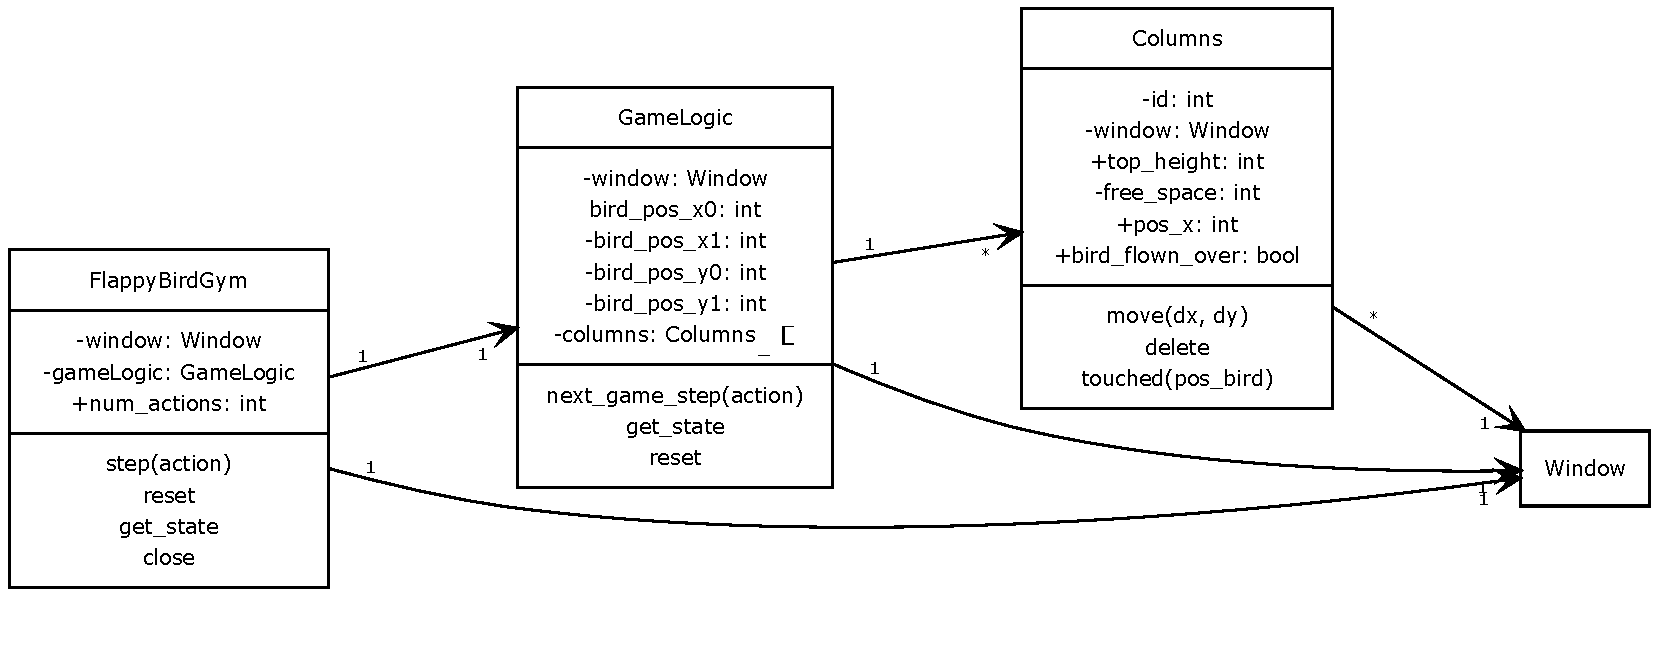
\includegraphics[width=\textwidth]{media/gym.pdf}
    \caption{Environment}
    \label{fig:uml-gym}
\end{figure}

A reference to the window object is passed to each of the mentioned classes. The \mintinline{python}{Window} class implements the graphical representation, which will be explained in further detail in section \ref{sec:ui}.

\subsubsection{Neural Network view}

Given this implementation of the game, what exactly does the state contain that is passed to the neural network? As it can be seen in 
listing \ref{listing:get-state}, for each state 12 parameters are passed to the ANN, which makes 24 in total, since we pass the current and the previous state. These describe the positions of the bird and the two columns which the bird has to pass next. For each of these elements, we pass four parameters, since they have the form of rectangles.
\begin{listing}[!ht]
\begin{minted}{python}
def get_state(self):
    return np.array([
        self.bird_pos_x0, self.bird_pos_y0,
        self.bird_pos_x1, self.bird_pos_y1,
        self.first_column.top_pos_x0, self.first_column.top_pos_y0,
        self.first_column.top_pos_x1, self.first_column.top_pos_y1,
        self.first_column.down_pos_x0, self.first_column.down_pos_y0,
        self.first_column.down_pos_x1, self.first_column.down_pos_y1
    ])
\end{minted}
\caption{get\_state}
\label{listing:get-state}
\end{listing}
The neural networks output is binary, either "flap" or "no flap". It is passed to the environment on each step.
% Network behaviour on a single frame
\subsubsection{Reward function}
In RL it is straightforward to define the outcomes but it is more difficult to define the way to get there.
For instance, in Flappy Bird it is uncomplicated to define how to win the game but it is more complicated to determine how the bird will fly to survive. The bird will simply fly as it rewarded for.
\par
In our reward function, we decided to give the neural network a bit more information than just the game score. In order to pass a gap between two pipes, the bird's vertical position must be between the lowest point of the upper pipe and the highest point of the lower pipe. We wanted to reward our network when this is the case and we did so in the form of a Gaussian reward function which is at it's maximum when the bird is right in the center of the gap.
\par


$reward(x)  
= \frac{\mathcal{N}(x|\mu, \sigma)}{\mathcal{N}(\mu|\mu, \sigma)}  
= \frac{\mathrm{}\frac{1}{\sigma\sqrt{2\pi}} \exp{\biggl(-\frac{(x - \mu)^{2}}{2\sigma^{2}} \biggr)}} 
{\mathrm{}\frac{1}{\sigma\sqrt{2\pi}} \exp{\biggl(-\frac{(\mu - \mu)^{2}}{2\sigma^{2}} \biggr)}}  
= \exp{\biggl(-\frac{(x - \mu)^{2}}{2\sigma^{2}} \biggr)}$

with 

$\mathcal{N}(x|\mu, \sigma) = \mathrm{}\frac{1}{\sigma\sqrt{2\pi}} \exp{\biggl(-\frac{(x - \mu)^{2}}{2\sigma^{2}} \biggr)} $
where  x is $bird\_posY0$; 
\par
Furthermore the reward function is normalized to be between 0 and 1 in order to prevent tiny q values. This is visualized in figure \ref{fig:Rewardsystem}.
\par
The two vertical ordered columns which are the nearest to the bird are considered for the reward calculation. µ denotes the y coordinate of the center of the space between these two columns. 
$\sigma$ denotes the scaled length in y direction of this space. In order to force the model to control the bird more towards the middle the length of the space is scaled by a factor of 0.125.
\begin{figure}
    \centering
    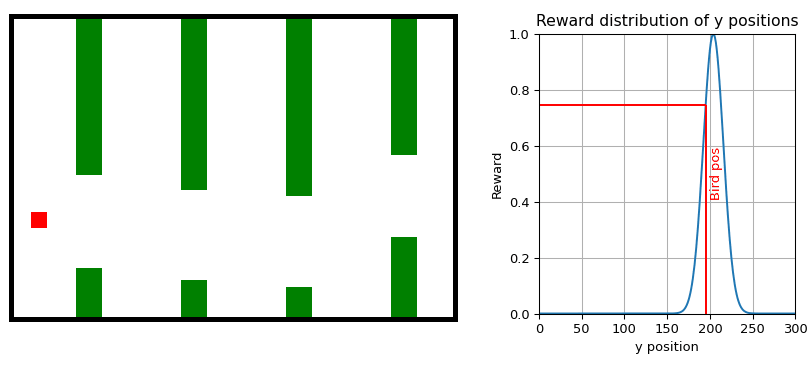
\includegraphics[width=\textwidth]{media/rewardSystem.png}
    \caption{Reward system}
    \label{fig:Rewardsystem}
\end{figure}


%!!Tim fragen wegen Grafik!!


\subsection{Neural Network}

When creating our neural network, we followed the structure we learned during the course. We created a subclass of \mintinline{python}{tf.keras.Model} and implemented the relevant methods \mintinline{python}{__init__}, \mintinline{python}{call} and \mintinline{python}{train_step}. 
% Network overview
\begin{listing}[!ht]
\begin{minted}{shell}
Layer (type)                 Output Shape              Param #   
=================================================================
dense (Dense)                multiple                  1600      
_________________________________________________________________
dense_1 (Dense)              multiple                  8320      
_________________________________________________________________
dense_2 (Dense)              multiple                  129       
_________________________________________________________________
dense_3 (Dense)              multiple                  258       
=================================================================
Total params: 10,307
\end{minted}
\caption{Network summary}
\label{listing:network-summary}
\end{listing}

Since our input data is a small array of numbers (and not the full graphical representation of the game), dense layers suffice to solve the given task (and we do not need any convolutional layers). Listing \ref{listing:network-summary} shows in detail which layers we used. Figure \ref{fig:model-plot} shows the complete network structure, including activation functions.

\begin{figure}
    \centering
    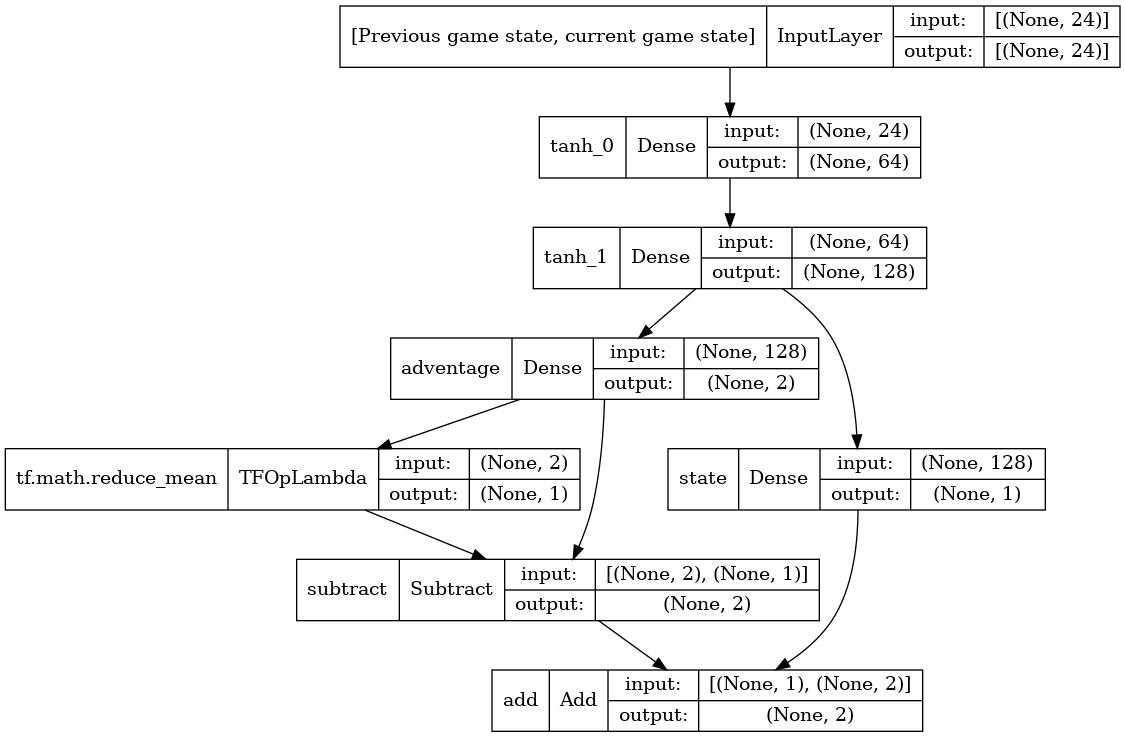
\includegraphics[width=\textwidth]{media/modelPlot.png}
    \caption{Model Plot}
    \label{fig:model-plot}
\end{figure}
\subsection{Hyperparameters}
An important task was to adjust the hyperparameters to obtain the best performance. The choices were not always trivial and we tried several approaches. 
By following the structures we learned in the course but also experimenting with different parameters, in the end we obtained the best performance using the hyperparameters presented in Listing \ref{listing:hyperparams}.


\begin{listing}[!ht]
\begin{minted}{python}

General:
    learning rate = 0.001
    optimizer = Adam
    loss function = mean squared error
    batch size = 32
EpsilonGreedyStrategy:
    start = 1.0 
    end = 0.05
    decay = 0.99 (multiplicative decay after each episode until end is reached)
ReplayMemory:
    capacity = 500.000
    num_samples = 250.000 # number until training the network starts
    sampling process: samples with higher reward preferred
Deep Q Learning:
    gamma = 0.99
    update = 100 # number of episodes when weights of qnet = weights of target net

\end{minted}
\caption{Hyperparameters}
\label{listing:hyperparams}
\end{listing}



\subsection{Double Deep Q-Learning}\label{sec:ddql}

Figure \ref{fig:uml-q-learning} shows how we implemented the Double Deep Q-Learning architecture to let our network learn Flappy Bird. The most superordinate class instance is \mintinline{python}{Training}. It runs the training loop and uses the wrapper classes \mintinline{python}{Agent} and \mintinline{python}{EnvManager} to access the network and the environment. The "Double" of Double Deep Q-Learning is realized by having two neural networks, \mintinline{python}{q_net} and \mintinline{python}{target_net}. In the following, we will describe how these two networks behave during the training loop in detail:
\begin{enumerate}
    \item Filling the replay memory. The untrained network plays the game until the replay memory is filled. When we trained the network, we set the size of the replay memory to 250000.
    \item For each episode:
    \begin{enumerate}
        \item Based on the current exploration rate (which decays over time) and a random value, chose whether the next step will explore or exploit.
        \item Perform a step based on the networks current parameters; if we are exploiting, chose the best option, if we are exploring, chose a random option.
        \item Store the whole step (state before action, action, state after action and reward) in the replay memory.
        \item Perform a training step: Select a sample from the replay memory. Predict the Q-values by both \mintinline{python}{q_net} and \mintinline{python}{target_net}. Compute the maximum Q-value of the next state using the \mintinline{python}{q_net}. The update operation differs a  bit from what we learned during the seminar: We take the action chosen by the \mintinline{python}{q_net} (the action that has the maximum Q-value) and add the expected reward predicted by the \mintinline{python}{target_net} for that exact action to the reward.
        \item Using the state and the computed Q-target (sum of rewards so far and the expected reward described in the previous point multiplied by the discount factor $\gamma$), we can perform a train step on the \mintinline{python}{q_net}.
        \item Repeat these steps for each episode 500 times. After this amount of steps, reduce the exploration rate.
    \end{enumerate}
    \item After 100 episodes, copy the current \mintinline{python}{q_net} to be the new \mintinline{python}{target_net}. In total, we run 5000 episodes.

\end{enumerate}
\par
\begin{figure}
    \centering
    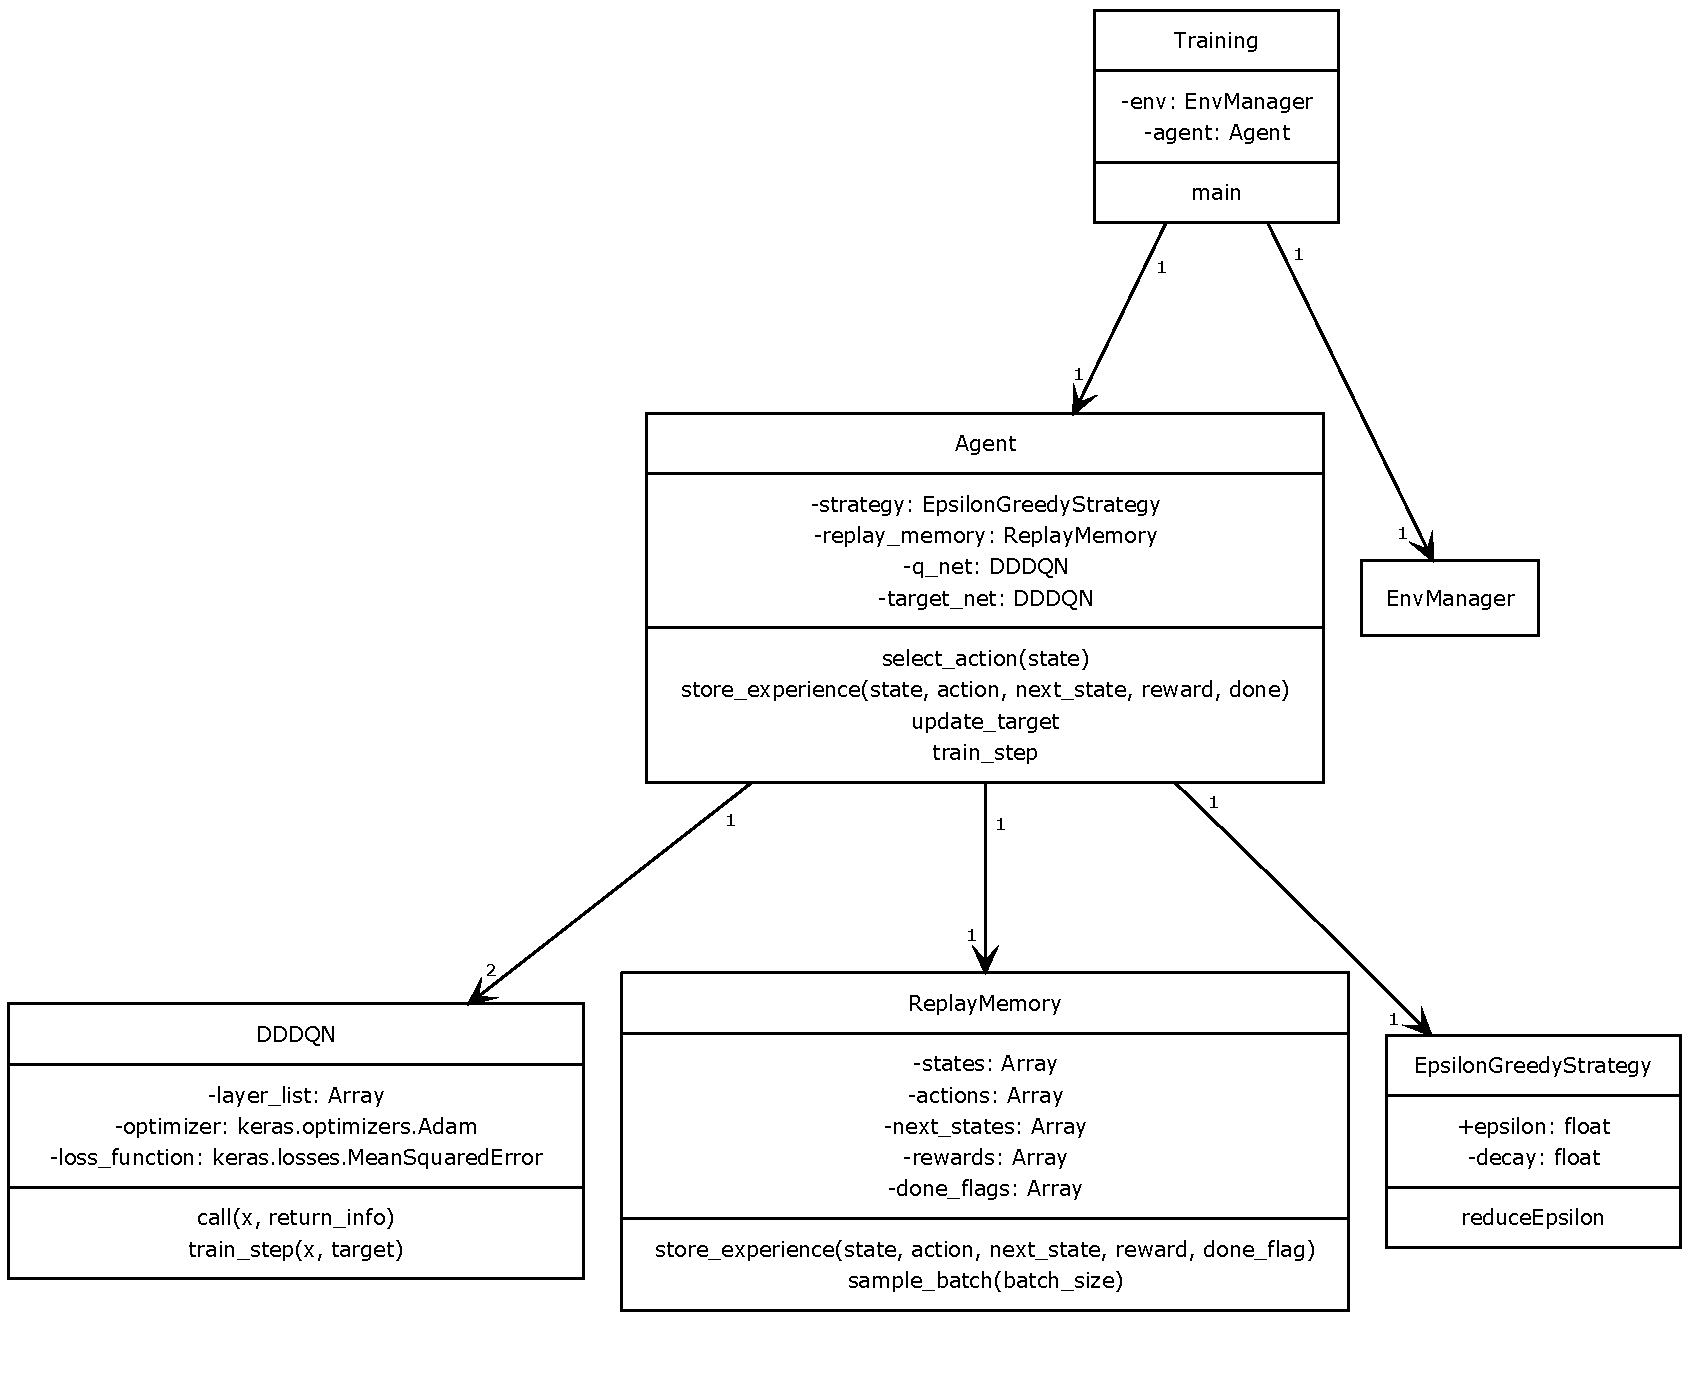
\includegraphics[width=\textwidth]{media/network.pdf}
    \caption{Double Deep Q-Learning}
    \label{fig:uml-q-learning}
\end{figure}


\subsection{User Interface}\label{sec:ui}

We developed three different modes of running our network:
\begin{enumerate}
    \item No window
    \item Game window
    \item Game + Stats window
\end{enumerate}
The no window-mode runs without GUI, although some information are passed to the user via command line. We used that mode for training, since it runs the fastest.
\par
The game window mode shows the actual game of Flappy Bird with the network-controlled bird. Compared to the no-window mode, the user can see how the bird is behaving, which can be used to troubleshoot problems if the network is not learning.
\par
Even more information are contained in the game + stats window mode (see figure \ref{fig:stats-window}), where in addition to the game itself also the internal game state and network behaviour is displayed. The top three plots show which action is currently seen as the best by the network, the current reward distribution in relation to the bird's height and the so far obtained rewards. In the bottom row, the UI shows the 12 inputs of the current state and the activations of the layers 1 and 2. On the left, we can see our graphical representation of the game itself which also looks the same in the game window mode.

\begin{figure}
    \centering
    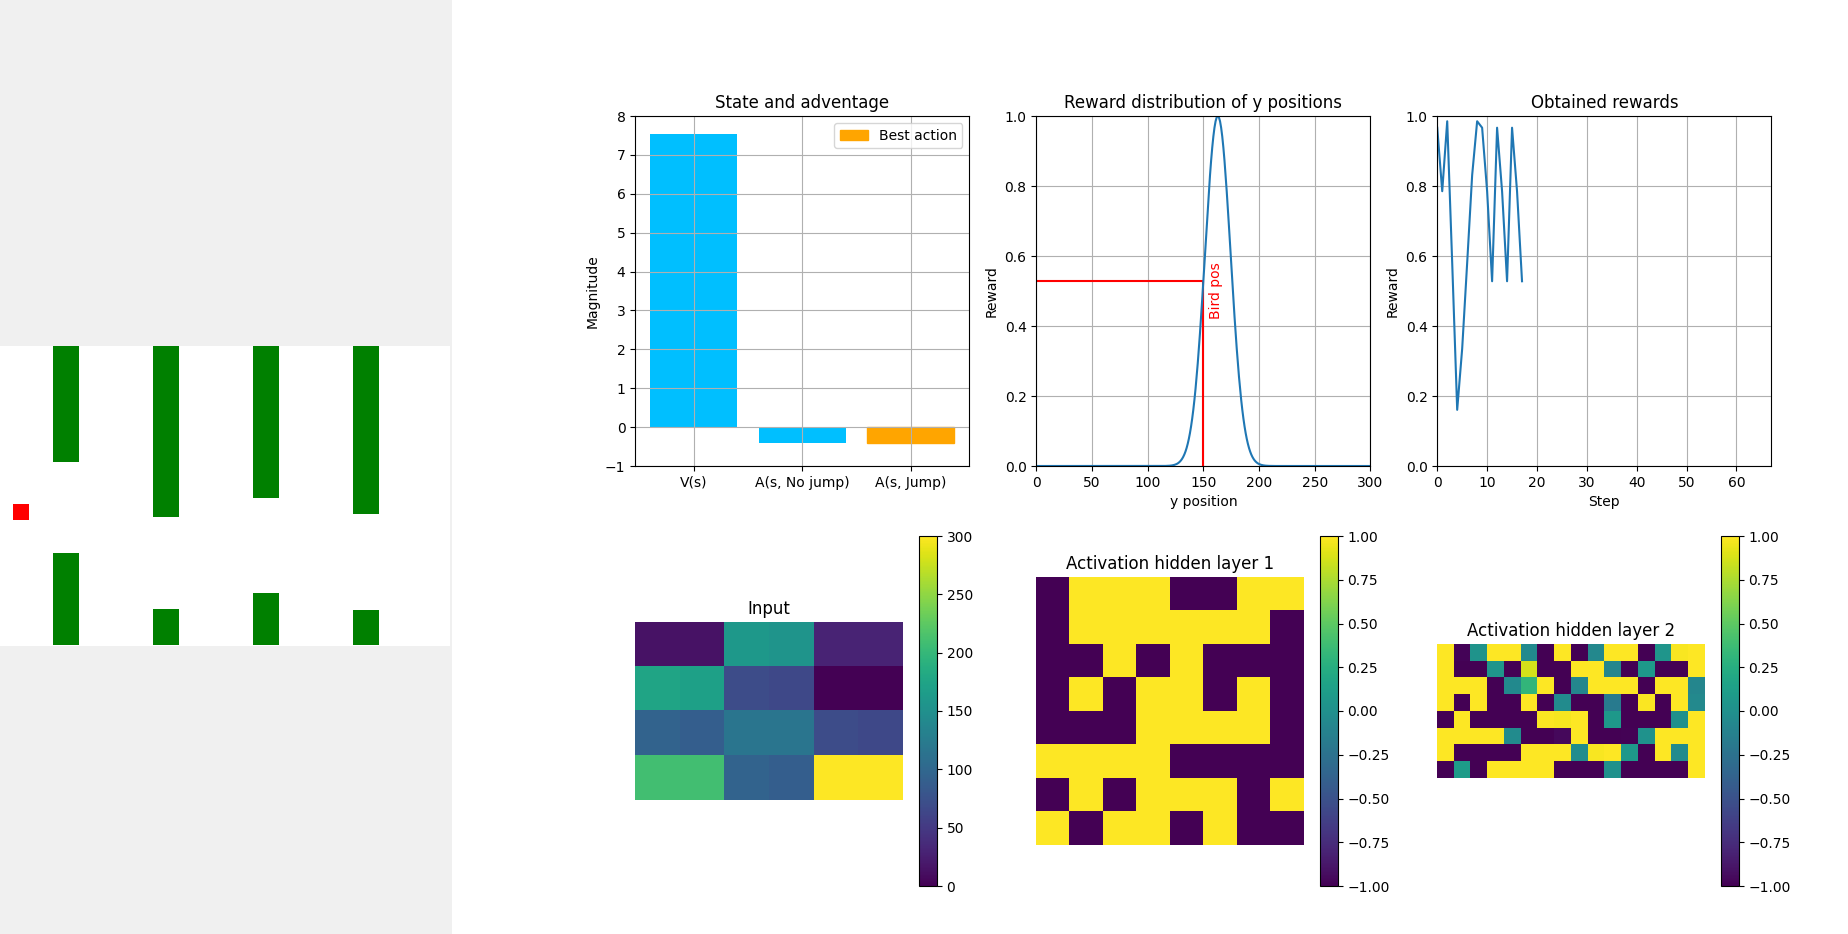
\includegraphics[width=\textwidth]{media/Screenshot-stats-window.png}
    \caption{Game + Stats Window Mode}
    \label{fig:stats-window}
\end{figure}
